\documentclass[12pt]{article}

\usepackage{sbc-template}

\usepackage{graphicx,url}

\usepackage[brazil]{babel} 
  
\usepackage[utf8]{inputenc}       

\usepackage{lipsum}

\sloppy

\title{Evoluç\~{a}o do Hardware dos consoles até o ano de 2000}

\author{Henrique Shodi Maeta e \\ Luiz Frederico Santos de Queiroz Junior}


\address{{Centro Universit\'{a}rio Senac, Santo Amaro}
\email{japa1996@hotmail.com luluiz21@hotmail.com}}

\begin{document} 

\maketitle
     
\begin{resumo}
Atualmente os consoles de video game já est\~{a}o bem difundidos, podendo ser o passa tempo preferido de algumas pessoas. Jogos s\~{a}o e foram feitos para todos poderem desfrutarem, sendo jogos educacionais, de estratégia, etc. Além de um bom passa tempo para a maioria das pessoas, isto pode ser também emprego para as pessoas que trabalham com video game, como os desenvolvedores, designers, gamers e streamers(que s\~{a}o profiss\~{o}es relativamente novas). Trataremos neste artigo sobre a evoluç\~{a}o dos consoles, mais especificamente ao hardware, até o ano 2000, desde os osciloscópios até o Nintendo64.
\end{resumo}


\section{Introdu\c c\~{a}o}

\ \ A história dos consoles começa quando os cientistas da computaç\~{a}o iniciam suas pesquisas nas áreas de Inteligencia artificial, simuladores, computaç\~{a}o grafica entre outros.
\begin{figure}[!h]
    \centering
    \includegraphics[width= 1\textwidth]{timeline.jpg}
    \caption{Linha do tempo dos consoles e jogos até o ano de 2009}
    \label{fig:timeline}
\end{figure}

Apesar dos arcades n\~{a}o aparecerem na linha do tempo, estes foram muito importantes para a evoluç\~{a}o da relaç\~{a}o entre os humanos e jogos, ser\~{a}o citados neste artigo.

\section{Pioneiros}
 O primeiro video game, segundo o artigo "From Pong to Playstation 3" \cite{pong-play} foi projetado em 1948 quando Thomas T. Goldsmith Jr. (americano pioneiro no ramo da televis\~{a}o e professor de física na Furman University) e Estle Ray Mann emitiram uma patente americana para um "Despositivo para divers\~{a}o de tubo de raios catódicos", que era uma maquina com uma maçaneta para mirar e um bot\~{a}o para atirar em alvos de avi\~{o}es inspirada no radar, um dispositivo usado na Segunda Guerra Mundial. Mas por conta do custo do equipamento este projeto nunca foi fabricado, apenas surgiram poucos protótipos de fabricaç\~{a}o caseira inspirados neste projeto.
 Dez anos após o primeiro projeto o físico americano William A. Higinbotham, que participou da equipe que desenvolveu a primeira bomba nuclear, criou o Tennis for Two (Tênis para dois), que era um jogo onde um computador analógico era adicionado a um ociloscópio:
\linebreak
\begin{figure}[!htb]
    \centering
    \includegraphics[width=0.8\textwidth]{osciloscopio.jpg}
    \caption{Imagem do jogo Tennis for Two no osciloscópio.}
    \label{fig:osciloscopio}
\end{figure}
\linebreak
 Os jogadores possuiam um bot\~{a}o para regular o ângulo que a bola iria seguir, e um bot\~{a}o para acertar a bola.
 
 Em 1961 um grupo de estudantes do MIT (Massachusetts Institute of Technology) escreveram o código de um jogo para o computador que eles possuiam DEC PDP-1(Figura \ref{fig:pc-velho}, página \pageref{fig:pc-velho}), que foi o primeiro computador comercial focado na interação com o usuário do que o uso convencional na época, que era utilizá-lo para ciclos computacionais, tal jogo foi nomeado Spacewar!(Figura \ref{fig:spacewar}, página \pageref{fig:spacewar}). O jogo se baseava em duas naves espaciais (jogadores) que atiravam, e, o objetivo era derrotar a nave do outro jogador. 
\linebreak
\begin{figure}[!htb]
    \centering
    \includegraphics[width=0.8\textwidth]{pc-velho.jpg}
    \caption{Computador DEC PDP-1 mesmo modelo que os alunos utilizaram para programar Spacewar!}
    \label{fig:pc-velho}
\end{figure}
\linebreak
\begin{figure}[!htb]
    \centering
    \includegraphics[width=0.6\textwidth]{spacewar.jpg}
    \caption{Imagem do jogo Spacewar!, onde os pontos verdes representam os jogadores.}
    \label{fig:spacewar}
\end{figure}
\linebreak

Os computadores não possuiam configurações como vemos hoje em dia, por motivos óbvios de desenvolvimento e, no início dos anos 70 ainda não existiam microprocessadores, e por conta disso, na época, equipamentos como memória de acesso randômico (RAM) e memória apenas para leitura (ROM) possuiam o preço muito elevado tornando assim a existência em máquinas de jogos quase que inviáveis. De acordo com o site computerhistory \nocite{pdp1} um modelo do PDP-1 poderia custar, na época em que foi lançado, em torno de \$120,000, ele possuia 4K de tamanho de memória em words(do inglês: palavras) podendo ser de 16K dependendo de sua vers\~{a}o, o tamaho da word era de 18-bits, em computadores modernos é comum os tamanhos de word serem de 32 ou de 64 bits. O PDP-1 era capaz de realizar 100,000 somas por segundo, seus métodos de entrada e saída eram uma máquina de escrever, rolo de papel, para armazenamento de dados, CRT que permitia os programadores escreverem e editarem seus programas, além de poder ser usada para jogar os jogos que nele eram programados, fita magnética, uma caneta de luz que, quando conectada ao dispositivo ou ao monitor, permitia que o usuário apontasse para a tela e fizesse desenhos ou ent\~{a}o selecionasse objetos, assemelhando-se ao touch-screen e ao mouse que possuímos hoje em dia. Foram produzidas apenas 50 unidades deste computador, cada um com um peso aproximado de 1200 lbs(544 kg aproximadamente).
\nocite{ram}
\section{Arcades}
No inicio de 1970 os jogos de fliperama ou arcades começaram a aparecer, incluindo uma vers\~{a}o do Spacewar! chamada ent\~{a}o de Computer Space, desenvolvido pelos empreendedores e engenheiros Nolan Bushnell e Ted Dabney que fundaram a empresa Atari em 1972. Tal empresa contava com apenas mais um engenheiro e eles trabalhavam com um laboratório bem modesto, segundo relato de Allan Alcorn, no artigo entitulado "First-Hand:The Development of Pong: Early Days of Atari and the Video Game Industry"\cite{allan}, engenheiro que trabalhou na Atari, o laboratório possuia apenas um osciloscópio velho.


Nesta época os arcades faziam sucesso porém a melhor época ainda estava por vir, pois no final dos anos 70 e no começo dos anos 80 o mercado dos arcades ja estava difundido, principalmente pela presença do famoso jogo Space Invaders(Figura \ref{fig:spaceinvaders}, página \pageref{fig:spaceinvaders}), Battlezone(Figura \ref{fig:battlezone}, página \pageref{fig:battlezone}), e o PAC-MAN(Figura \ref{fig:pacman}, página \pageref{fig:pacman}). O mercado de arcades nessa época movimentava em torno de \$5,000,000 apenas na América do Norte.

\begin{figure}[!ht]
    \centering
    \includegraphics[width=0.4\textwidth]{spaceinvaders.jpg}
    \caption{Imagem da tela do arcade, com o jogo Space invaders.}
    \label{fig:spaceinvaders}
\end{figure}
\begin{figure}[!htb]
    \centering
    \includegraphics[width=0.4\textwidth]{battlezone.jpg}
    \caption{Imagem do jogo Battlezone.}
    \label{fig:battlezone}
\end{figure}
\begin{figure}[!ht]
    \centering
    \includegraphics[width=0.4\textwidth]{pacman.jpg}
    \caption{Imagem do famoso jogo PAC-MAN.}
    \label{fig:pacman}
\end{figure}
\newpage

Em quest\~{a}o de Hardware, os arcades eram computadores dedicados a rodarem apenas jogos, num sistema totalmente unificado, ou seja, sem periféricos adicionais, apenas os bot\~{o}es de comando, sendo que no início, um sistema de arcade rodava apenas o jogo que nele era programado. Apenas anos após o lançamento dos arcades foram desenvolvidas placas na qual o hardware era separado do software, como os da SEGA, CAPCOM, NAOMI, entre outros.
\begin{figure}[!ht]
    \centering
    \includegraphics[width=0.5\textwidth]{placaarcade.jpg}
    \caption{Placa do sistema de um Arcade.}
    \label{fig:placaarcade}
\end{figure}

\section{Consoles}
\subsection{Magnavox Odyssey}

A ideia de um video game para se jogar em casa veio em 1950, na mente de Ralph Baer(inventor, engenheiro alem\~{a}o), enquanto o mesmo trabalhava em um equipamento para TV em Nova York. Porém a ideia n\~{a}o foi muito aceita no momento em que Baer a apresentou a empresa contratante Loral Corporation. Até que em 1968 Baer e seus colegas finalizaram um protótipo do projeto, que foi nomeado Brown Box(caixa marrom Figura \ref{fig:prototipo}, página \pageref{fig:prototipo}), e o apresentaram à empresa Sanders Associates na cidade de Nashua, New Hampshire.

Em 1971 o console foi licenciado para Magnavox, e depois foi renomeado para Magnavox Odyssey(Figura \ref{fig:magna}, página \pageref{fig:magna}), e só em maio de 1972 o console foi disponibilizado para o público. Vendendo mais de 340.000 unidades, sendo a linha mais rentável da Sanders.

O Odyssey não continha processador e nem memória. A caixa era feita de transinstores, resistencias e condensadores. As paletas de cores eram em preto e branco, o áudio era RF. Existiam dois espaços para controles, que eram do tipo "paddle" (controle analógico baseado em um potenciômetro) (Figura \ref{fig:controle}, página \pageref{fig:controle})
\begin{figure}[!htb]
    \centering
    \includegraphics[width=0.3\textwidth]{prototipo.jpg}
    \caption{Brown Box criado por Ralph Baer e seus colegas, este protótipo se encontra em Smithsonian Institution.}
    \label{fig:prototipo}
\end{figure}
\begin{figure}[!htb]
    \centering
    \includegraphics[width=0.4\textwidth]{magna.jpg}
    \caption{Vers\~{a}o comercializada do Magnavox Odyssey.}
    \label{fig:magna}
\end{figure}
\begin{figure}[!htb]
    \centering
    \includegraphics[width=0.4\textwidth]{controlemag.jpg}
    \caption{Controle tipo paddle.}
    \label{fig:controle}
\end{figure}
\newpage
\subsection{Fairchild Channel F}
Em novembro de 1976 a empresa Fairchild Semiconductor lançou o Video Entertainment System, ou VES, que mais tarde, em 1977 viria a se chamar  Fairchild Channel F, quando a Atari lança seu VCS. Este console foi muito importante para história pois foi o primeiro a utilizar a memória ROM(read only memory, memória apenas para leitura), permitindo com que o jogo fosse pausado, e também foi o primeiro com um microprocessador. 

O Fairchild Channel F possuía um controle simples, e 26 jogos em fitas, incluindo boliche, corrida, entre outros. Seu sucesso foi muito curto. Pssuia um processador de 1.79 MHz possuia 64 bytes de momória RAM, trabalhava com a paleta de 8 cores, cada midia tinha capacidade de 4 KB e a resoluç\~{a}o era de 128x64. Cada unidade do Fairchild Channel F custava aproximadamente \$169.
\begin{figure}[!htb]
    \centering
    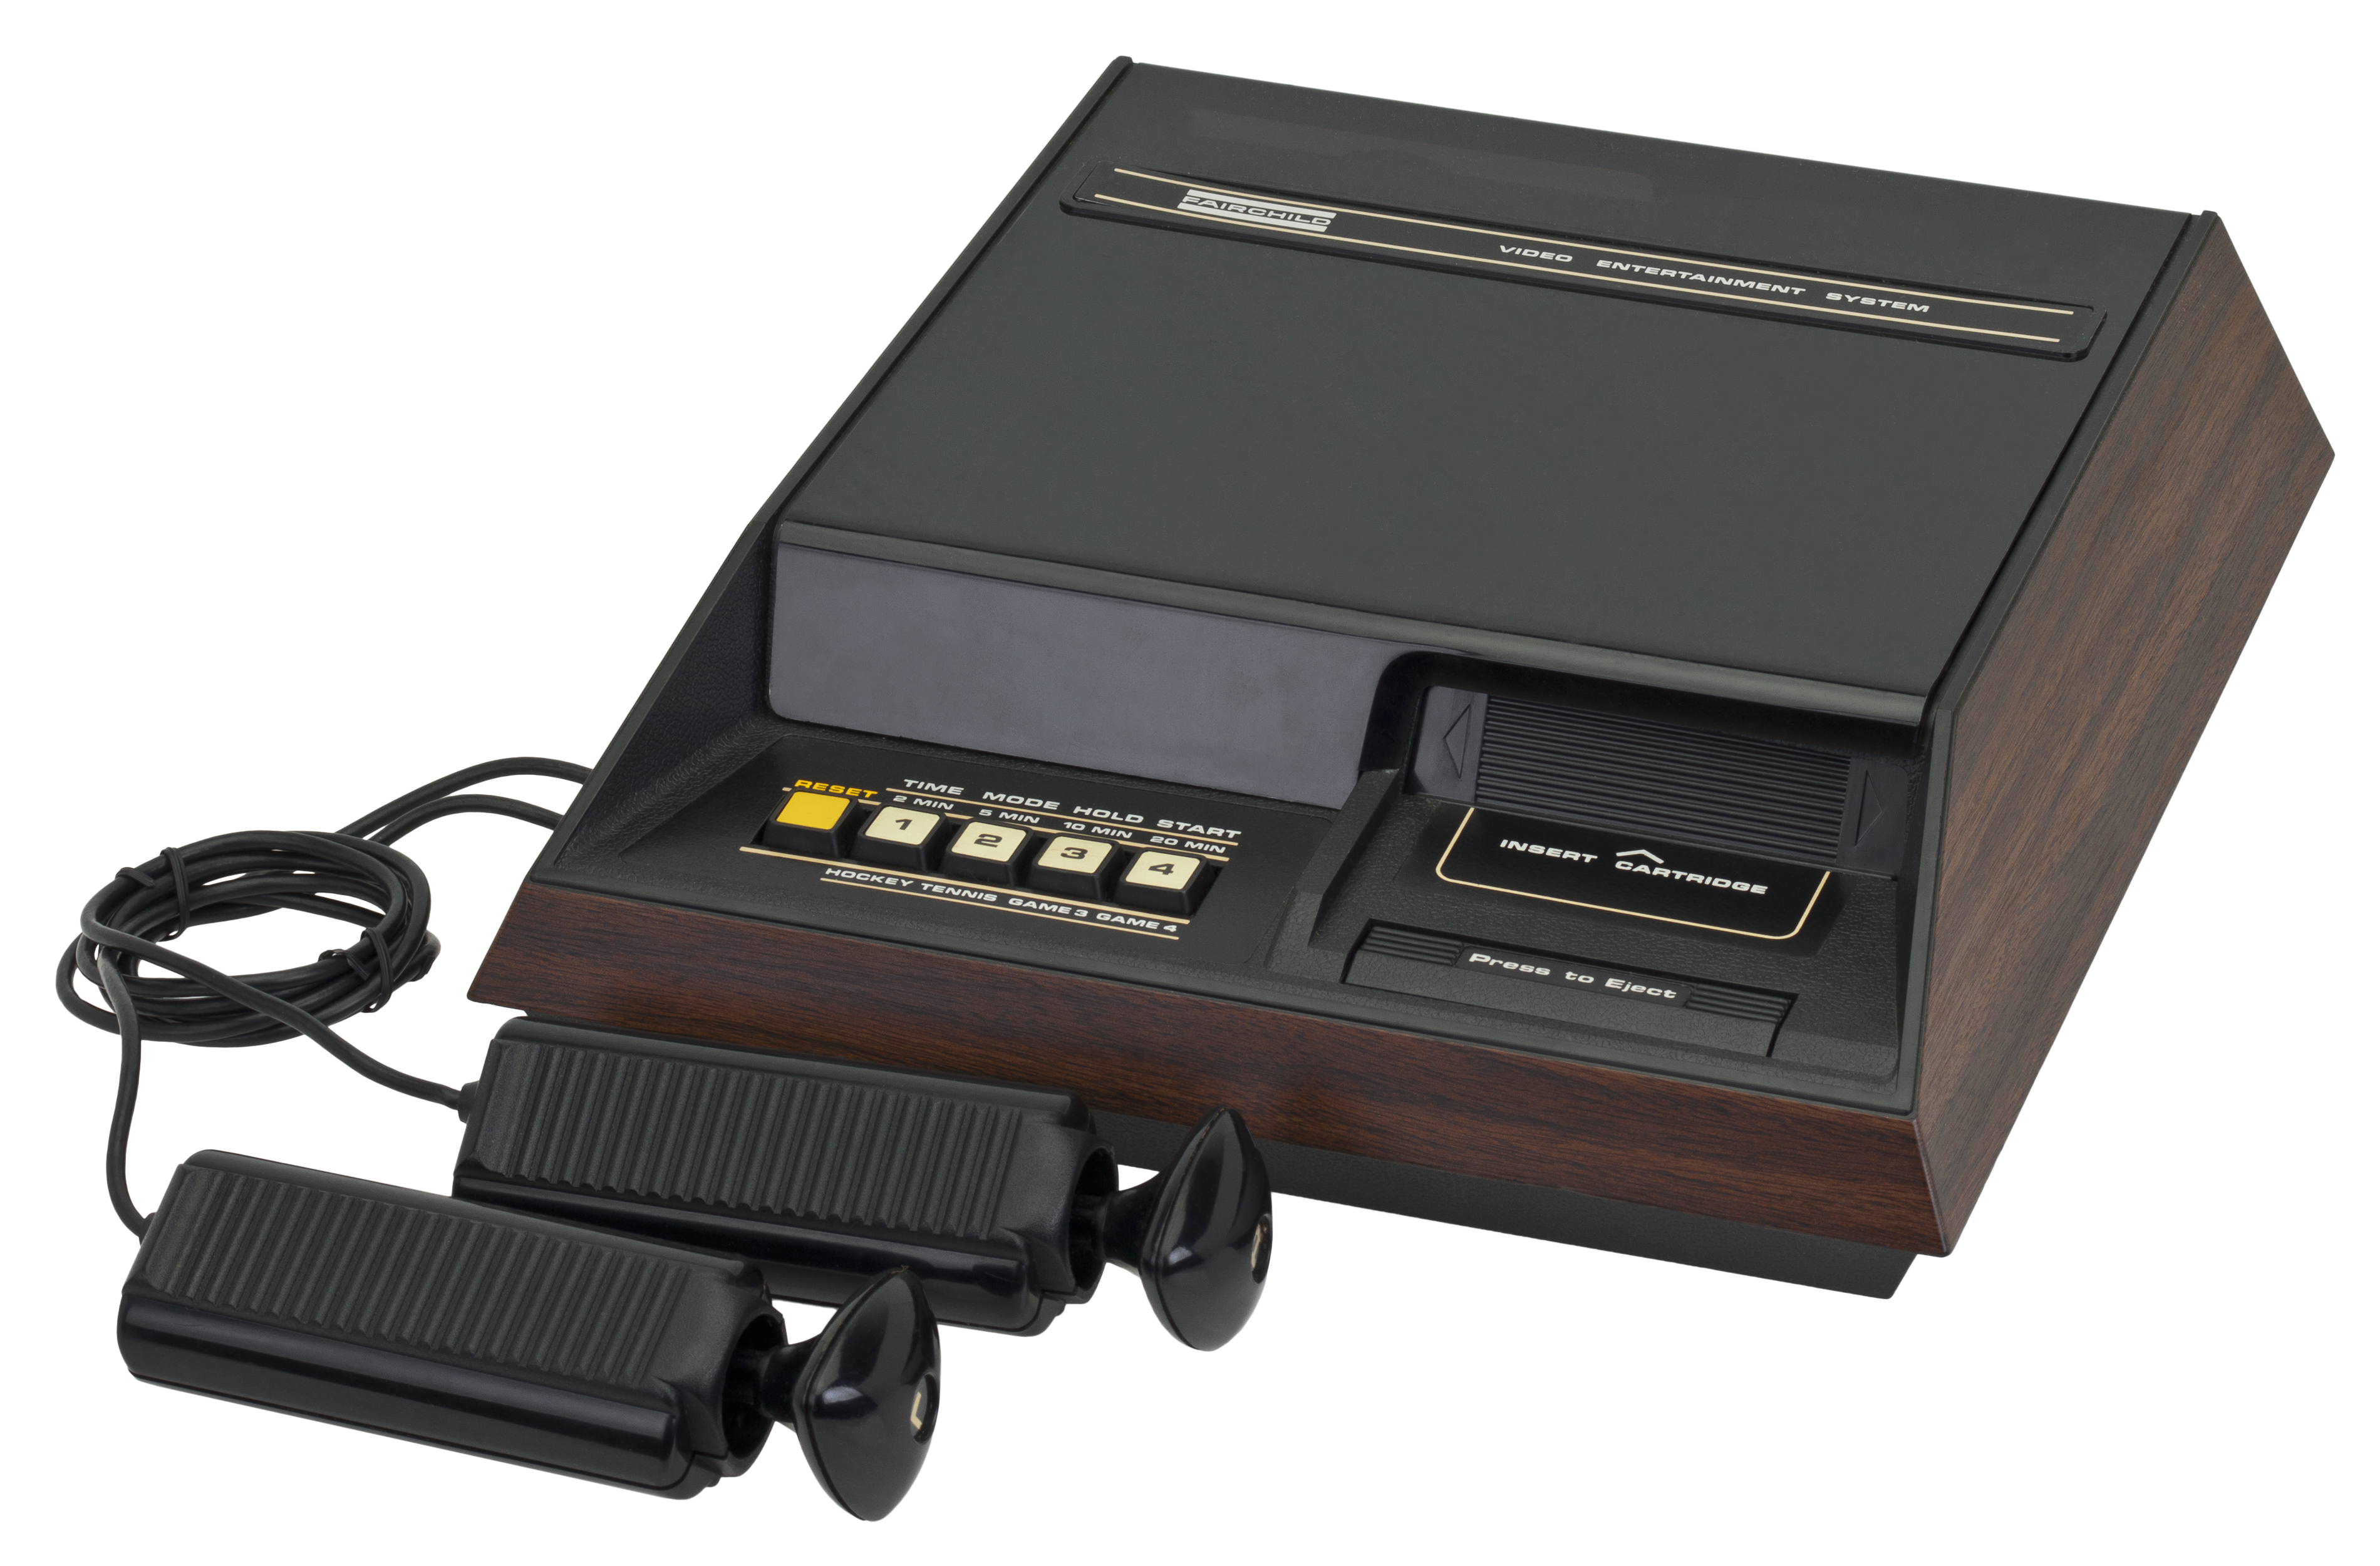
\includegraphics[width=0.3\textwidth]{VES.png}
    \caption{Fairchild Channel F e seus controles}
    \label{fig:controle}
\end{figure}

\subsection{Atari 2600}
Ted Dabney and Nolan Bushnnell criaram a Atari gaming system em 1970, que atuava pelo nome "Syzygy". Apenas em 1972 eles mudaram o nome da compania para "Atari". Em 1973, Atari tinha comprado uma empresa de engenharia chamada Cyan Engineering para desenvolver um sistema de nova geração, e trabalhou em um protótipo conhecido como "Stella". Diferente de máquinas de gerações passadas que usavam lógica de programação própria e fixa para rodar um pequeno número de jogos, o núcleo do Stella era um CPU completo.

O dono da Atari, Steve Bushnell, percebeu que não teria fundos suficientes para que eles concluíssem o ambicioso projeto, então ele vendeu a Atari para a Warner Communications. O projeto então decolou e quando foi lançado se chamou Atari 2600 ou Atari Video Computer System, nome mais usado para fins de marketing.

O sistema contava com um micro-processador de 1.19 Mhz e 8-bits. A memória RAM era de apenas 128 bytes, para manter os custos de produção baixos. Claro que isso dificultou e muito a programação dos jogos. Os desenvolvedores tiveram que fazer milagre para permitir que os games rodassem nos 128 bytes de memória. O primeiro "truque" usado é que os jogos eram carregados diretamente a partir da ROM (o código não era copiado para a memória RAM como atualmente), o que liberava a memória RAM para ser usada em variáveis e pequenos blocos de código que precisavam de execução rápida.
 
Como o chip TIA 1A não oferecia memória de vídeo, a atualização da tela não podia ser feita usando um frame-buffer (em outras palavras, não pra armazenar uma cópia da imagem na memória de vídeo como se faz hoje). Aproveitando o fato de que o Atari era ligado na TV (que trabalha com uma taxa de atualização fixa de 30 Hz interlaçados), os projetistas criaram um sistema engenhoso, onde a imagem era atualizada linha a linha, em um processo contínuo, onde o processador precisava armazenar apenas alguns poucos bytes relacionados aos pixels seguintes.

O Atari 2600 (Figura \ref{fig:atari}, página \pageref{fig:atari}) possui um processador 8 bits com velocidade de 1.19 MHz, 128 bytes de memória ram. Resolução de 320x200, 128 cores (16 cores x 8 variações). Áudio com dois canais, mono. Mídia com formato de cartucho com capacidade de até 4KB. Capacidade para dois controles( joystick com um botão ).

 \begin{figure}[!htb]
    \centering
    \includegraphics[width=0.5\textwidth]{atari.jpg}
    \caption{Atari 2600}
    \label{fig:atari}
\end{figure}

\subsection{Nintendo Entertainment System}
O NES foi lançado oficialmente nos EUA no dia 18 de Outubro de 1985 apenas em Nova York, para teste de aceitação do público. Foram disponibilizadas inicialmente 50.000 unidades que se esgotaram rapidamente, o que levou a Nintendo a lançar o console no resto do país em Fevereiro do ano seguinte. Mais tarde o console foi lançado oficialmente na Europa, Austrália e Brasil. O sistema, apesar da concorrência com o Sega Master System, manteve-se na liderança dos mercados japonês e americano durante uma década.

O NES (Figura \ref{fig:nes}, página \pageref{fig:nes}) possui um processador de 8 bits, a velocidade é de NTSC: 1,79 MHz e PAL: 1,66 MHz. 2 KB de Ram e video. Resolução de tela 256 x 240, paleta de cores com 52( 25 na tela), possui 64 sprites. Áudio PSG Som (5 Canais) Mono. Formato da mídia é cartucho com capacidade de 1 Mib. Capacidade para dois controles (D-Pad, 2 botões de ação, Start \& botões Select). 

 \begin{figure}[!htb]
    \centering
    \includegraphics[width=0.5\textwidth]{nes.jpg}
    \caption{NES}
    \label{fig:nes}
\end{figure} 

\subsection{Master System}
 O Master System(Figura \ref{fig:system}, página \pageref{fig:system}).Lançado inicialmente no Japão em 1986, com o nome Sega Mark III, ele enfrentou grandes dificuldades devido à forte concorrência do NES da Nintendo.A Nintendo possuía contratos de exclusividade junto às produtoras de jogos. O contrato não permitia que elas produzissem jogos para nenhum outro aparelho, fazendo com que o Master System dependesse quase que somente dos lançamentos desenvolvidos pela Sega.
 
 Master sytem possui um processador de 8 bits de velocidade 3.58 MHz (NTSC) \ 3.54 MHz (PAL). Memória ram de 8 KB e video 16 KB. Resolução 256x224 (NTSC) \ 256x240 (PAL). Paleta de cor 64 cores(32 na telas), posssui 16 sprites. Áudio 4 canais, mono. Mídia no formato de cartucho ( 256KB) e cartão de jogo sega(32Kb). Tinha capacidade para dois controles(D-Pad (8-direçoes), dois botões de ação.
 
 \begin{figure}[!htb]
    \centering
    \includegraphics[width=0.5\textwidth]{masters.jpg}
    \caption{Master System}
    \label{fig:system}
\end{figure} 

\subsection{Mega Drive}
Mega Drive(Figura \ref{fig:mega}, página \pageref{fig:mega}),lançado oficialmente em 1988) conhecido como Sega Genesis na América do Norte, é um console de video game de 16 bits da Sega que concorria diretamente com o Super Nintendo Entertainment System com 29 milhões de copias vendidas. O console fez grande sucesso na década de 1990, perdendo espaço após o surgimento e popularização da nova geração de consoles de 32 bits, como o PlayStation da Sony.

Possuia um processador de de 16 bits com velocidade de 7,67 MHz (NTSC) 
de 7,61 MHz (PAL). Com 64 KB de memória RAM e Video Ram. Resolução de tela podendo varia entre essas 256x224, 256x448, 320x224, 320x448. Paleta de com 512 cores(64 na tela), com 80 sprites. Formato de mídia é um cartucho com capacidade de 4 MB( até 10 MB com mapeador de memória). Armazenamento interno 2KB ROM (boot). Tem capacidade para 2 controles (D-pad(16 direções) botão iniciar e 3 botões de ação).

\begin{figure}[!htb]
    \centering
    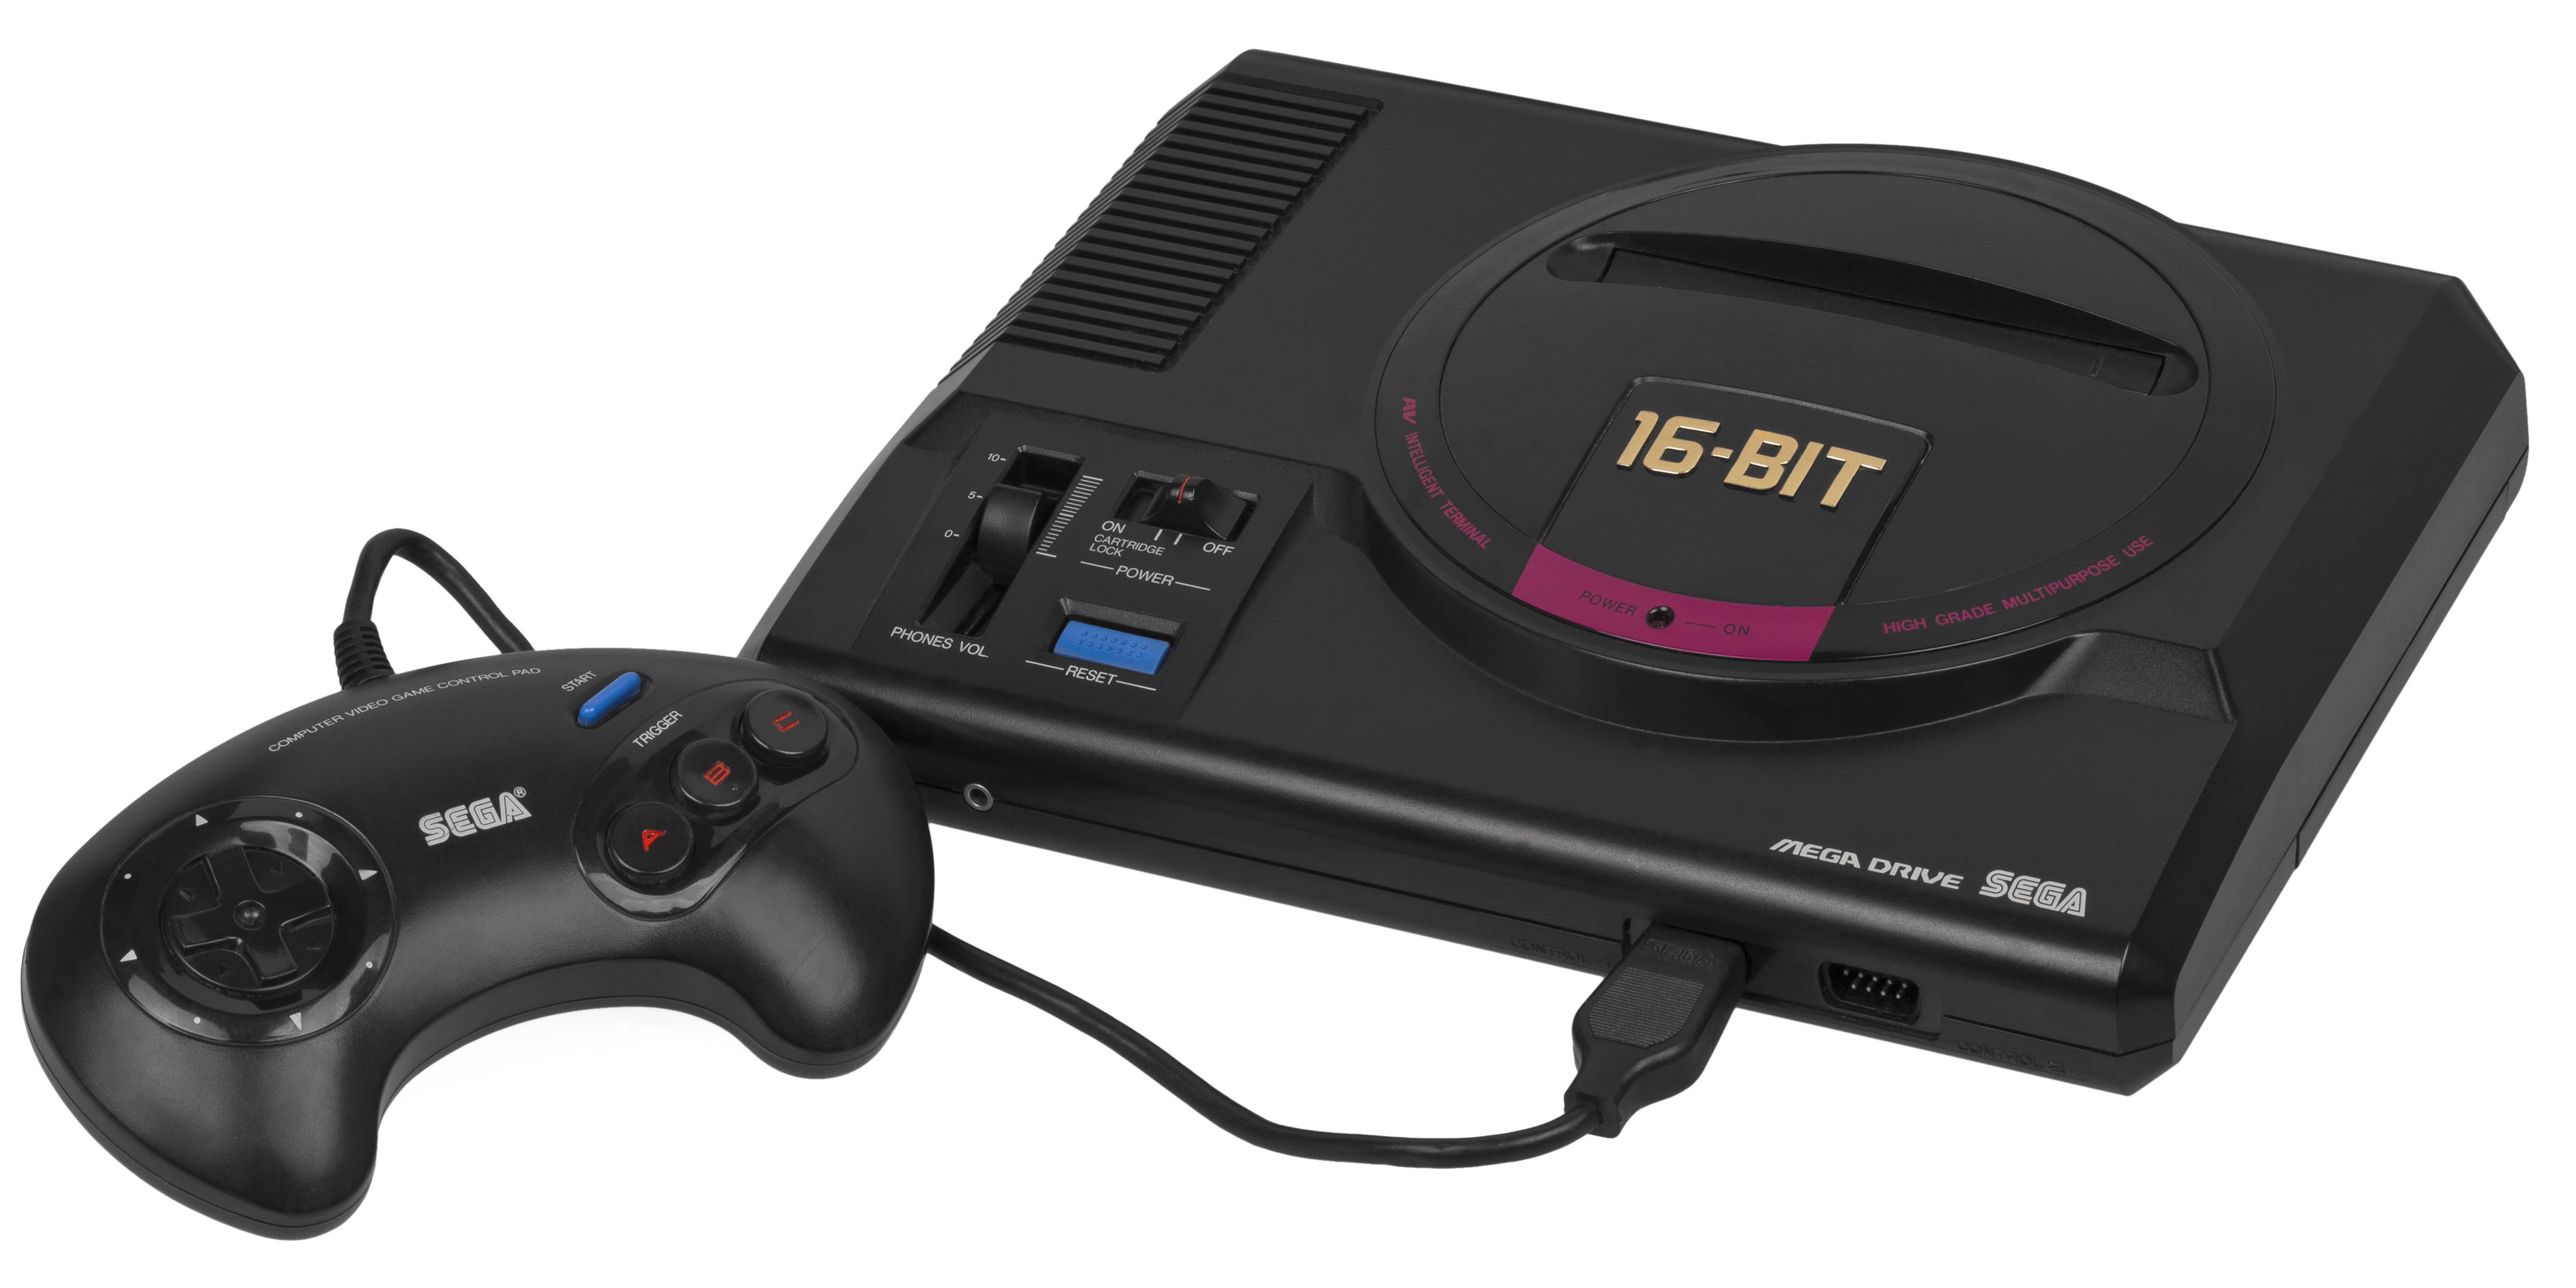
\includegraphics[width=0.5\textwidth]{megadrive.png}
    \caption{Mega Drive}
    \label{fig:mega}
\end{figure} 



 \subsection{Super Nintendo Entertainment System}
 O Super Nintendo Entertainment System (Figura \ref{fig:snes}, página \pageref{fig:snes})(abreviado oficialmente como Super NES ou ent\~{a}o SNES) foi um console com o processador de 16-bits criado pela Nintendo que sucedeu o NES, uma empresa japonesa, que leva seu nome. Foi lançado, em sua vers\~{a}o japonesa e sul-coreana, no ano de 1990, 1991 na América do Norte, 1992 na Europa e na Austrália e em 1993 na América do Sul. Mesmo sendo o mesmo video game, muitos bloqueios de regi\~{a}o os tornavam incompatíveis uns com os outros. Comparado com os consoles da época o Super NES possuía graficos avançados e capacidade de som elevada. Foram vendidas, no mundo inteiro, aproximadamente 41 milh\~{o}es de unidades, com um preço médio de \$210
\nocite{SNES}
\begin{figure}[!htb]
    \centering
    \includegraphics[width=0.5\textwidth]{SNES.jpg}
    \caption{Super NES americano.}
    \label{fig:snes}
\end{figure} 
Ele contava com um processador de 3.58 MHz em sua vers\~{a}o NTSC e 3.55 MHz na PAL, 128 KB DRAM e 64 KB SRAM, trabalhava com paleta de 8-bits (256 cores), utilizava cartuchos de 14.8 MB, sua resoluç\~{a}o máxima era de 512 x 478 para no máximo 2 jogadores (D-Pad, 6 bot\~{o}es de aç\~{a}o, bot\~{o}e Select \ Start).


\subsection{Sony Playstation}
\nocite{sony}
A Sony tinha um contrato com a Nintendo para produzir um leitor de CD-ROM para o Super NES, porém o acordo foi quebrado. Ent\~{a}o  Ken Kutaragi, engenheiro, convenceu os executivos da Sony a darem continuidade ao projeto. Ken Kutaragi decidiu fazer um console com o processador de 32-bits, que utilizava CD-ROM ao invés dos cartuchos que eram muito comuns na época, que fosse fácil de programar, barato e ainda sim potente.

Foi assim lançado ent\~{a}o o Sony Playstation(Figura \ref{fig:play1}, página \pageref{fig:play1}) em 1994 no Jap\~{a}o e em 1995 nos Estados Unidos cado console custava cerca de \$300, vendo assim, até o ano de 2006(quando o console foi descontinuado pela empresa) 103 milh\~{o}es de unidades.


\begin{figure}[!htb]
    \centering
    \includegraphics[width=0.5\textwidth]{play1.jpg}
    \caption{Sony Playstation, também conhecido como Play 1.}
    \label{fig:play1}
\end{figure}

O Playstation contava com uma paleta de 32-bits, seu tipo de midia era CD-ROM com capacidade de 700MB, memória externa de 1 MB (também chamado de Memory Card), memória interna de 512 KB para o sistema operacional, 2 MB de memória RAM e 1 MB de Video RAM,  o processador trabalhava com um motor de geometria 3D com a frequência de 33.8688 MHz, resoluç\~{a}o de 256x224 até 640x480, renderizava 360 mil poligonos por segundo, suportava dois jogadores, o controle possuía D-Pad, 8 bot\~{o}es de aç\~{a}o e bot\~{o}es Start \ Select.
\linebreak

\subsection{Nintendo 64}
Nintendo 64 (Figura \ref{fig:n64}, página \pageref{fig:n64})(abreviado como N64) é o terceiro console de Video-game doméstico da empresa japonesa Nintendo. Lançado em 23 de junho de 1996 no Japão e em 29 de setembro nos EUA. Teve 32,93 milhões de unidades vendidas.O Nintendo 64 ficou conhecido por ser um console que oferecia a melhor experiência multiplayer, graças a sua capacidade de aceitar 4 controles simultâneos sem ajuda de acessório.

Ele possuia um processador de 64 bits com velocidade de 93,75 MHz 93 MIPS 4 MB RAMBUS RDRAM (expansível até 8 MB). Resolução de tela variada entre 256 x 224, 320 x 240 e 640 x 480. Paleta de cores com 16,8 milhões(32.000 na tela).Era capaz de renderizar 800 mil poligonos por segundo. Áudio de 48 kHz, 16-bit. Foi o último console a utilizar cartucho que tinha capacidade entre 4 MB e 64MB. Tinha capacidade de 4 controles(10 botões, uma alavanca analógica direcional, porta de extensão)
\begin{figure}[!htb]
    \centering
    \includegraphics[width=0.5\textwidth]{N64.jpeg}
    \caption{Nintendo 64}
    \label{fig:n64}
\end{figure}

\section{Consideraç\~{o}es Finais}
A intenção deste artigo é especificar a evolução dos consoles baseando nos detalhes de hardware, e com uma pequena introdução as histórias de cada consoles e de suas empresas. Os consoles estão cada vez mais presentes no cotidiano das pessoas. E está deixando de ser apenas um instrumento de lazer. Estão gerando empregos direta e indiretamente, como campeonatos de e-sports e sendo utilizados como ferramentas para videos. 

Os consoles evoluiram de maneira incrível, no início era muito básico, com aç\~{o}es básicas de movimentação. Com passar do tempo foram ganhando sons, motores gráficos melhores e conquistando mais fãs. Com o aumento da busca desse entreterimento as empresas começaram a competir e começar uma "corrida" de desenvolvimento para que pudessem fazer o console que mais agradace o público.



\bibliographystyle{sbc}
\bibliography{sbc-template}
\nocite{pc-velho}
\end{document}
